\appendix
\renewcommand\thefigure{A.\arabic{figure}}
\renewcommand\thesection{\Alph{section}}
\renewcommand{\thealgocf}{A.\arabic{algocf}}
\renewcommand\thetable{A.\arabic{table}}
\setcounter{section}{0}
\setcounter{algocf}{0}
%\renewcommand\thealgorithm{A.\arabic{algorithm}}
\setcounter{figure}{0}
\setcounter{table}{0}

\section{Appendix}
\label{s:appendix}

\subsection{Other Details}
\label{ss:optimizations}

Our \sysname{} implementation combines techniques from various sources to achieve high-quality, low-latency volumetric video streaming. We describe these briefly.

\parab{Stream Synchronization.}
%
WebRTC does not permit embedding frame numbers in video streams.
%
Following prior work~\cite{salsify}, the \sysname{} sender embeds a (pre-generated) QR code in each 4K depth and color tiled frame that encodes the frame sequence number (\cref{fig:tiled-view}).
%
The receiver decodes the QR code to obtain frame sequence numbers.
%
If both depth and color frames have not been decoded by the time necessary to render the point cloud, \sysname{} simply skips the frame.

\parab{Receiver-side rendering.}
%
The receiver must reconstruct point clouds from received 4K frames.
%
To do this, it needs the parameters and positions of the RGB-D cameras; these are exchanged once during connection setup or whenever they change.
%
The receiver uses these to transform the position of each pixel from each 4K frame into the global coordinate frame.
%
Together with the corresponding color attributes, these constitute the reconstructed point cloud at the receiver.
%
This point cloud may be more dense than necessary and may have more points because \sysname{} transmits a guard-band around the frustum (\cref{ss:view-prediction-and-culling}).
%
To speed up rendering, \sysname{} first voxelizes the point cloud, then culls the point cloud further to the actual (current) frustum, following prior work~\cite{vivo,groot}.

\parab{Pipelining and parallelism.}
%
To ensure frame-rate processing, \sysname{} consists of several stages that run in parallel, and each stage incurs a delay per frame of less than one inter-frame interval.
%
The sender has 4 stages: capture, view generation, tiling, and transmission.
The receiver also has 3 stages: receiving and synchronization, point cloud reconstruction, and rendering.
%
%% \raj{We say culling in receiver. This culling is receiver side culling to remove redundant points sent due to guard band before rendering. The audience might be confused if we suddenly say culling in receiver. May be not say about culling in the receiver? Only call the stage `point cloud reconstruction'.}
%
Thus, the total end-to-end \textit{processing} latency is within 180~ms.
%
Each stage has a dedicated thread, which is connected to the next stage by a small inter-stage buffer (implemented using a thread-safe queue).
%
We also employ parallelism within some stages when possible: \textit{e.g.}, view generation, and point cloud generation.

\parab{Minimizing the impact of packet loss.}
%
We enable several WebRTC features, including negative acknowledgments, Picture Loss Indication (PLI), and Full Intraframe Request (FIR).
%
Because 4K videos are large, the default Linux UDP socket buffer (213~KB) proved insufficient, so we increased it.

\subsection{Validating Design Choices}\label{s:just-design-choic}

\parab{Depth Encoding.}
\begin{figure}[t]
  \centering 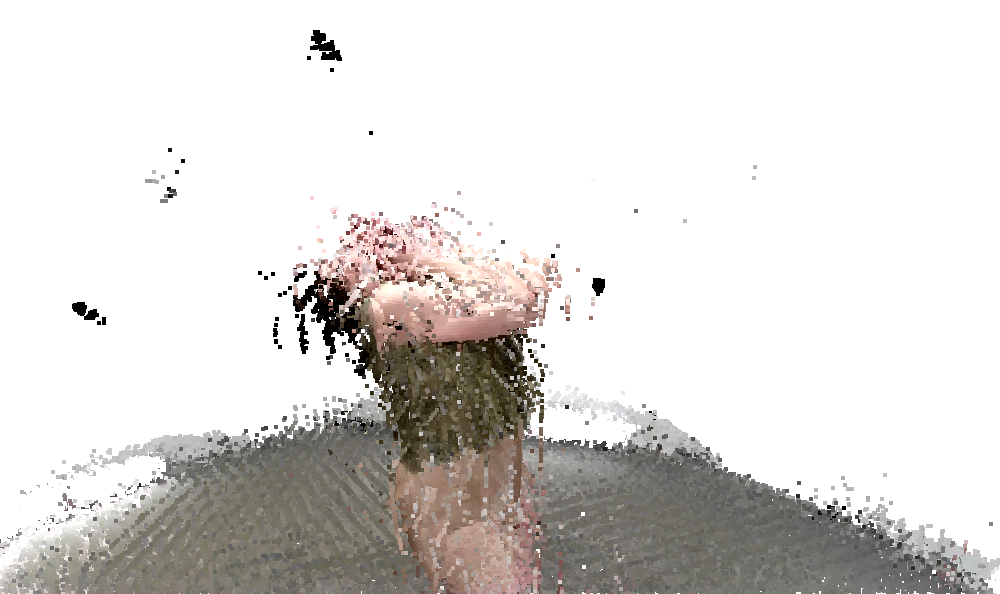
\includegraphics[width=\columnwidth]{figures/depth_unscaled_artifact.png}
  \caption{Block artifacts arising from unscaled depth encoding when we use naive H.265 YUV 16-bit variant.}
  \label{fig:depth-unscaled-artifact}
\end{figure}
%
\sysname encodes in Y-channel (luminance) of 3 channel 16-bit variant of H.265 encoding (Y444\_LE).
%
If the depth values aren't scaled to the full range, they produce artifacts as seen in \cref{fig:depth-unscaled-artifact}.
%
These artifacts arise since nearby depth values are mapped to same quantization bin within the 16-bit range.
%
So \sysname scales the depth values.
%
We also experimented with a strategy proposed by prior work~\cite{realsense-doc,depth-kautz,vrcomm} which colorizes each 16-bit depth pixel into a 3-channel RGB pixel using a depth to color conversion table.
%
\cref{plot:compression-choice} shows that \sysname{}'s scaled depth encoding achieves the highest geometry and color PSSIM relative to this approach and to unscaled depth encoding.

%% is significantly better than encoding depth in RGB, and that depth scaling is necessary to improve quality.
% %
% When we implement this strategy inside \sysname and apply to \textit{dance5} video, the average PointSSIM quality drops below 20 for both color and depth, which indicates severe quality degradation.
% %
% In contrast, naive strategy of putting depth in Y-channel (luminance) of 3 channel 16-bit variant of H.265 encoding (Y444\_LE Unscaled), improves PointSSIM geometry to above $70$.
% %
% Through visual inspection, we observed that the decoded point cloud have local block-like artifacts, which indicates that the neighbouring points have collapsed in one of the 3D dimensions (example in Appendix \cref{s:appendix}).
% %
% Our depth encoding strategy using depth scaling improves both PointSSIM color and geometry to reach 90.

\begin{figure}[tbp]
  \centering 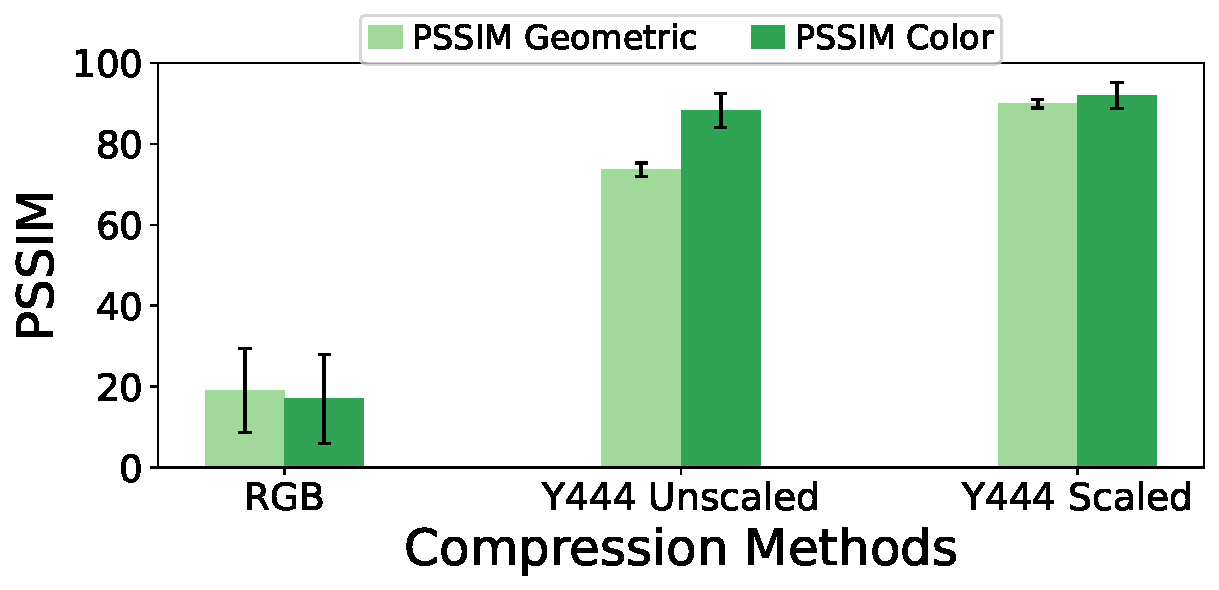
\includegraphics[width=0.5\columnwidth]{figures/pssim_compression_comparison.pdf}
  \caption{Comparison between realsense vs our approach.}
  \label{plot:compression-choice}
\end{figure}

%\harsha{Suggest moving the para below and associated table to appendix.}
\parab{Kalman Filter buffer size.}
%
Kalman filter prediction error depends on the prediction horizon.
%
\sysname targets prediction horizons of about 10 frames (300~ms).
%
Predictions help culling, which can reduce data volume, but erroneous predictions can impact quality.
%
\sysname uses a static guard-band $\epsilon$ of 20~cm around the frustum to minimize quality loss due to prediction errors.
%
\cref{tab:prediction_acc} shows that for guard-bands up to 30~cm, \sysname's accuracy and data volume are relatively insensitive to the choice of guard-band, hence a static guard-band works well.
%
We have verified this for other videos as well.

% Prediction window is the number of lookahead frames between the last received frustum from receiver and the frustum required (through prediction) for the current outgoing frame on the sender.
% %
% We predict the frustum by running the Kalman Predictor same number of times as the prediction window size.
% %
% To correct for prediction errors, we use a guard band $\epsilon$ around the predicted frustum.
% %
% \cref{tab:prediction_acc} shows that for any prediction window size, the prediction accuracy increases with increase in the guard band size, but it comes at a cost.
% %
% Increased size of guard band results in large fraction of points in the full point cloud to fall inside the frustum; refer~\cref{tab:prediction_fraction}.
% %
% This increases unnecessary transmission of data at reduced quality.
% %
% We observe that \sysname achieves an end-to-end latency <300~ms, which corresponds to a prediction window size of 10 frames (at 30~FPS).
% %
% From \cref{tab:prediction_acc}, we observe that increasing guard band size above 20~cm have marginal improvements in prediction accuracy, while saving $40\%$ of the points from transmission.
% %
% Thus, we choose $\epsilon$ to be 20~cm in \sysname.

\begin{table}[t]
\centering
  \footnotesize
  \scalebox{0.8}{
    \begin{tabular}{|l|l|l|l|l|}
    \hline
    \multicolumn{1}{|l|}{\multirow{2}{*}{\textbf{\begin{tabular}[c]{@{}l@{}}Guard \\ Band\end{tabular}}}} & \multicolumn{4}{c|}{\textbf{Prediction Window Size}} \\ \cline{2-5} 
    \multicolumn{1}{|l|}{} & \multicolumn{1}{l|}{\textbf{W=5}} & \multicolumn{1}{l|}{\textbf{W=10}} & \multicolumn{1}{l|}{\textbf{W=20}} & \multicolumn{1}{l|}{\textbf{W=30}} \\ \hline
    10 & 98.44 (0.57) & 96.69 (0.54) & 94.37 (0.57) & 91.76 (0.57) \\ \hline
    20 & 99.26 (0.62) & 98.37 (0.62) & 96.13 (0.62) & 93.95 (0.62) \\ \hline
    30 & 99.61 (0.66) & 98.97 (0.66) & 97.22 (0.67) & 95.41 (0.67) \\ \hline
    50 & 99.89 (0.73) & 99.56 (0.73) & 98.46 (0.73) & 97.18 (0.73) \\ \hline
    \end{tabular}
    }
    \caption{Accuracy  of culling using Kalman Filter by varying the guard band (in cm) for \textit{band2}. The numbers in brackets represent fraction of points within frustum.}
    \label{tab:prediction_acc}
\end{table}

% \begin{table}[t]
% \centering
%   \footnotesize
%     \begin{tabular}{|l|l|l|l|l|}
%     \hline
%     \multicolumn{1}{|l|}{\multirow{2}{*}{\textbf{\begin{tabular}[c]{@{}l@{}}Guard Band\\ (in cm)\end{tabular}}}} & \multicolumn{4}{c|}{\textbf{Prediction Window Size}} \\ \cline{2-5} 
%     \multicolumn{1}{|l|}{} & \multicolumn{1}{l|}{W=5} & \multicolumn{1}{l|}{W=10} & \multicolumn{1}{l|}{W=20} & \multicolumn{1}{l|}{W=30} \\ \hline
%     10 & 0.57 & 0.54 & 0.57 & 0.57 \\ \hline
%     20 & 0.62 & 0.62 & 0.62 & 0.62 \\ \hline
%     30 & 0.66 & 0.66 & 0.67 & 0.67 \\ \hline
%     50 & 0.73 & 0.73 & 0.73 & 0.73 \\ \hline
%     \end{tabular}
%     \caption{Fraction of points within the frustum by varying guard band size for `band2' video.}
%     \label{tab:prediction_fraction}
% \end{table}

% \begin{figure}[t]
%  \begin{minipage}[t]{0.49\columnwidth}
%    \centering
%     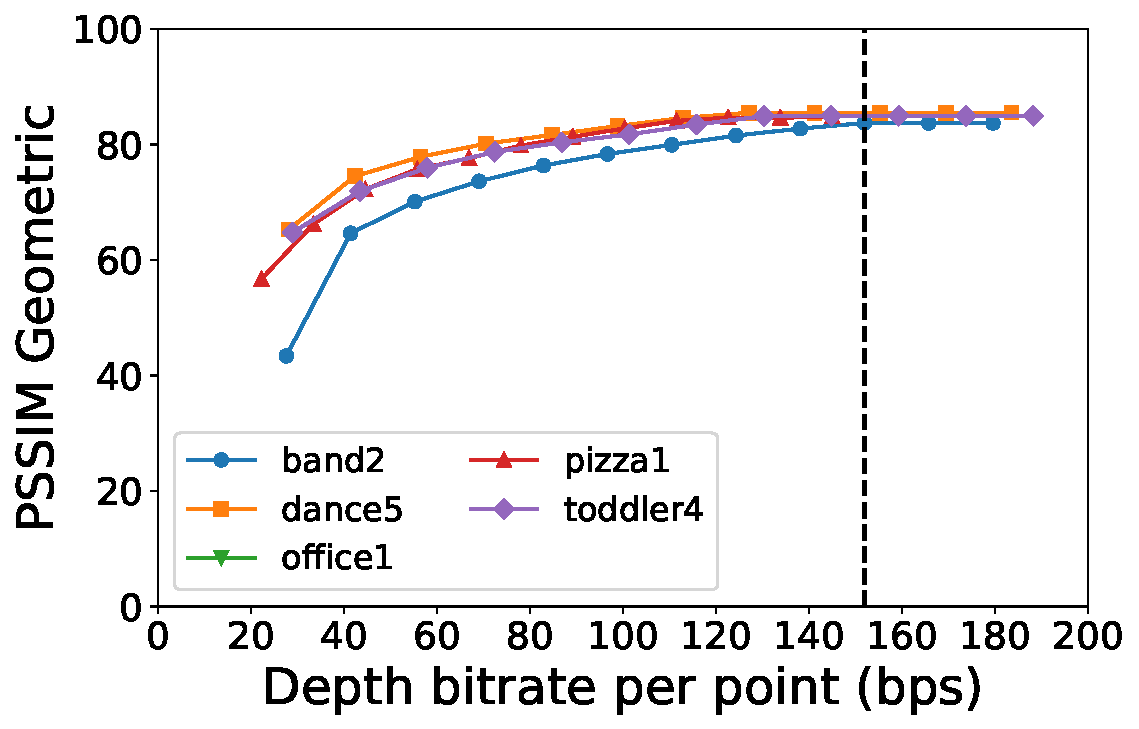
\includegraphics[width=\columnwidth]{figures/pssim_geometric_depth_per_point.pdf}
%    \caption{Depth distortion. \note{[Remove]}}
%    \label{plot:depth-distortion}
%  \end{minipage}
%  \begin{minipage}[t]{0.49\columnwidth}
%    \centering
%     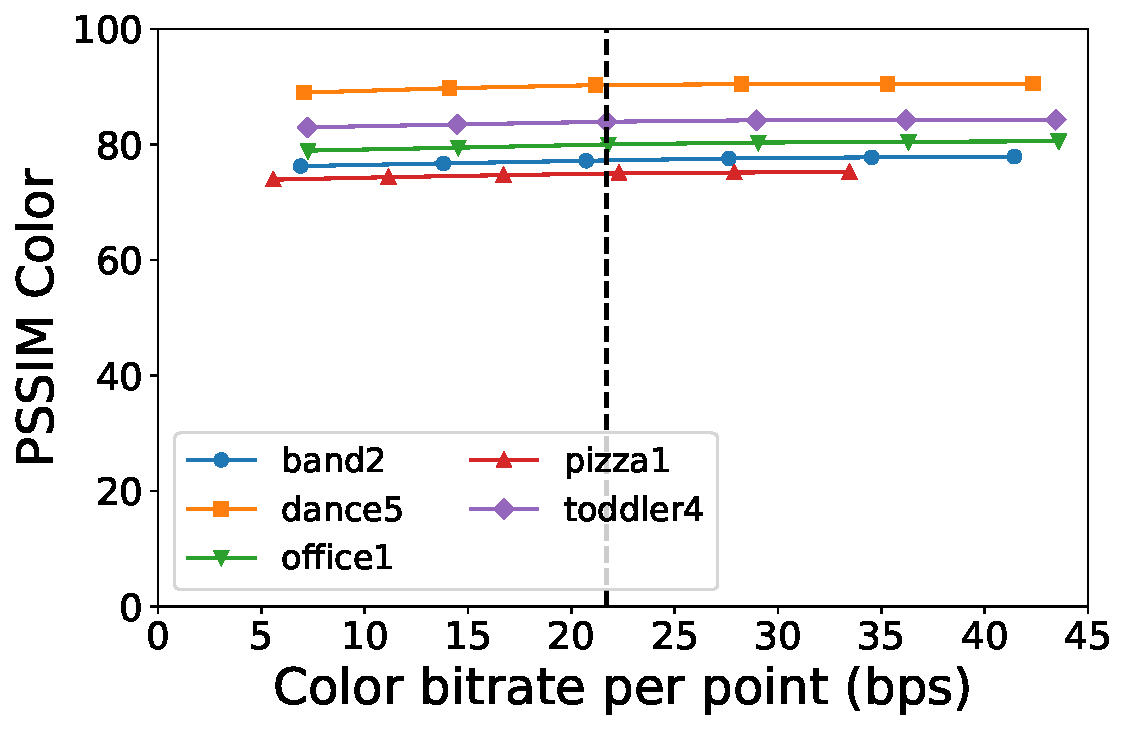
\includegraphics[width=\columnwidth]{figures/pssim_color_color_per_point.pdf}
%    \caption{Color distortion. \note{[Remove]}}
%    \label{plot:color-distortion}
%  \end{minipage}
% \end{figure}

\begin{figure}[t]
  \begin{minipage}[t]{0.49\columnwidth}
	    \centering
	     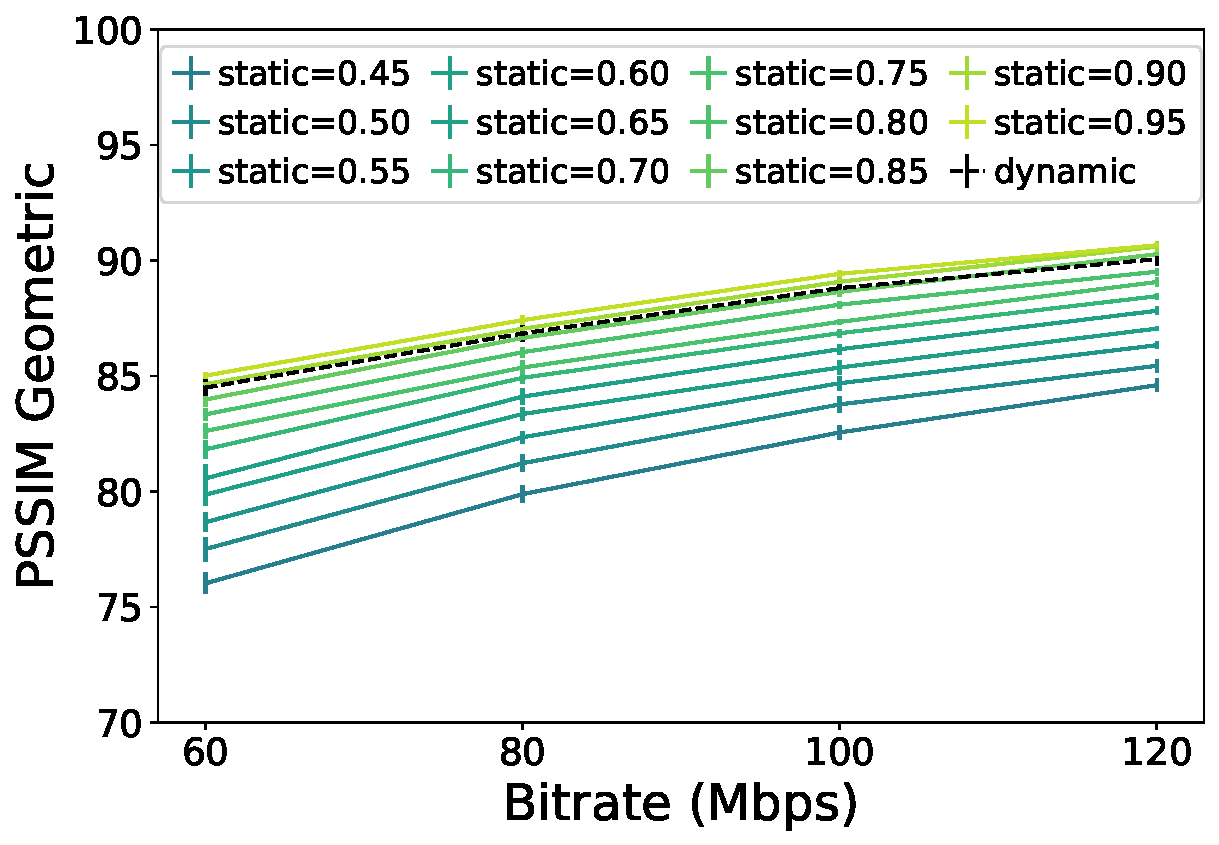
\includegraphics[width=\columnwidth]{figures/static_vs_dynamic_pssim_geo.pdf}
	    \caption{PSSIM Geometric for static vs dynamic split.}
	    \label{plot:split-sweep-geo}
	  \end{minipage}
  \begin{minipage}[t]{0.49\columnwidth}
	    \centering
	     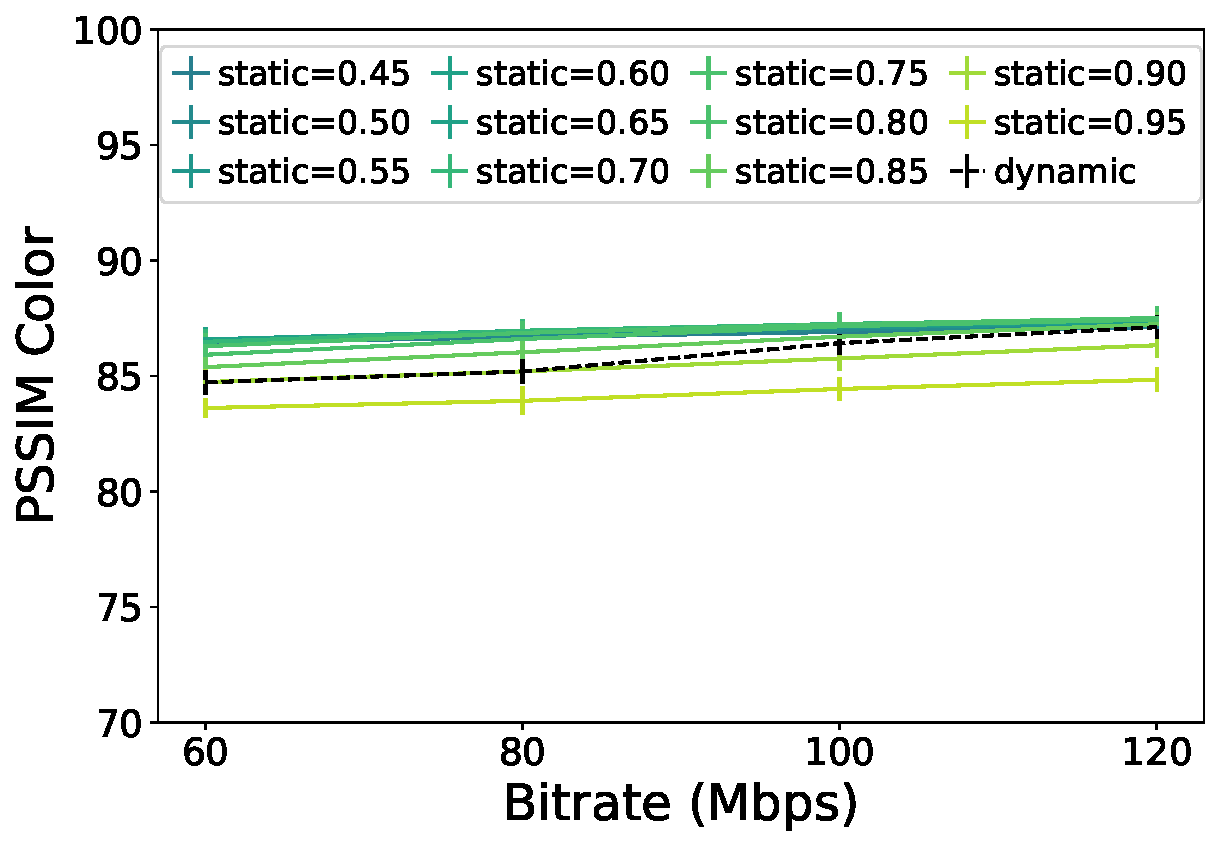
\includegraphics[width=\columnwidth]{figures/static_vs_dynamic_pssim_color.pdf}
	    \caption{PSSIM Color for static vs dynamic split.}
	    \label{plot:split-sweep-color}
	  \end{minipage}
\end{figure}

%% \begin{figure}[t]
%% 	\centering 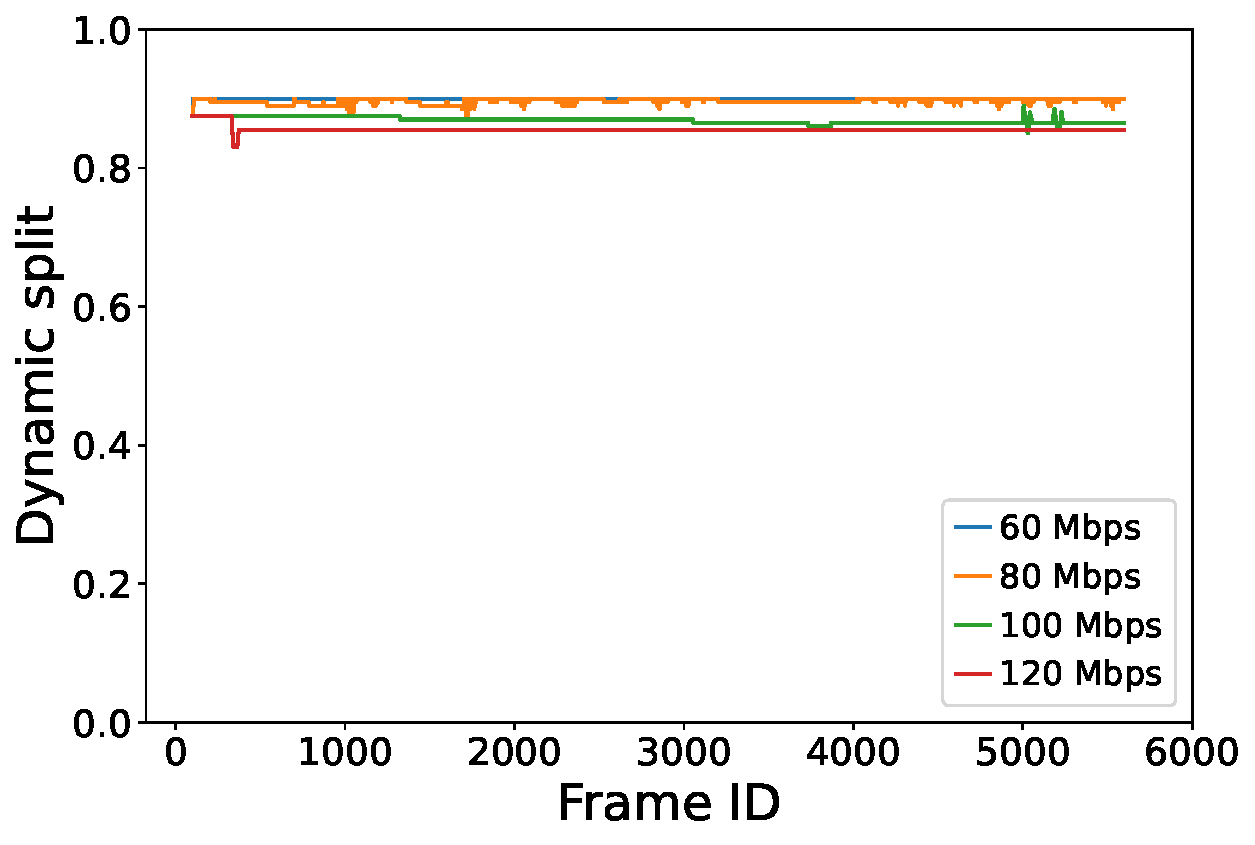
\includegraphics[width=0.5\columnwidth]{figures/split_convergence.pdf}
%% 	\caption{Split convergence.}
%% 	\label{plot:split-convergence}
%% \end{figure}

\parab{Bandwidth Splitting.}
%
%\cref{plot:depth-distortion} plots depth PSSIM as a function of bits per second per point, when color is assigned a high (100~Mbps) rate.
%
%Across all our videos, depth quality saturates at about 152 bits per second per point.
%
%Conversely, when depth bit rate is fixed, color PSSIM saturates at about 22 bits per second (\cref{plot:color-distortion}).
%
%Perceptual quality in 3D is more sensitive to depth encoding than color, since loss in depth leads to geometrical errors that can distort a 3D representation of an object.
%
%This justifies our choice of 7:1 as the ratio of depth to color per point.
%
\cref{plot:split-sweep-geo} plots compares PSSIM for different static splits with \sysname{}'s dynamic split (\cref{ss:bw-adaptation}) for bitrates ranging from 60-120~Mbps for \textit{office1} (similarly, color in \cref{plot:split-sweep-color}).
%
Dynamic splitting is with 0.5 PSSIM points for geometry and 3 PSSIM points for color relative to the best static split.
%
As available bandwidth increases, both geometry and color PSSIM values are within 0.5 of the best static split.
%
This demonstrates the effectiveness of dynamic splitting.
%
%% \cref{plot:split-convergence} shows how quickly the bitrate split converges when the scene complexity changes. 
%
Moreover, dynamic splitting converges quickly, within 5-10 frames (figure omitted for brevity).
%
%Also, the split variation occurs more for bandwidth limited than bandwidth adequate regions.
%

\parab{Bandwidth Adaptation.}
%
% \begin{figure}[t]
%      \centering
%      \begin{subfigure}[b]{0.49\columnwidth}
%          \centering
%          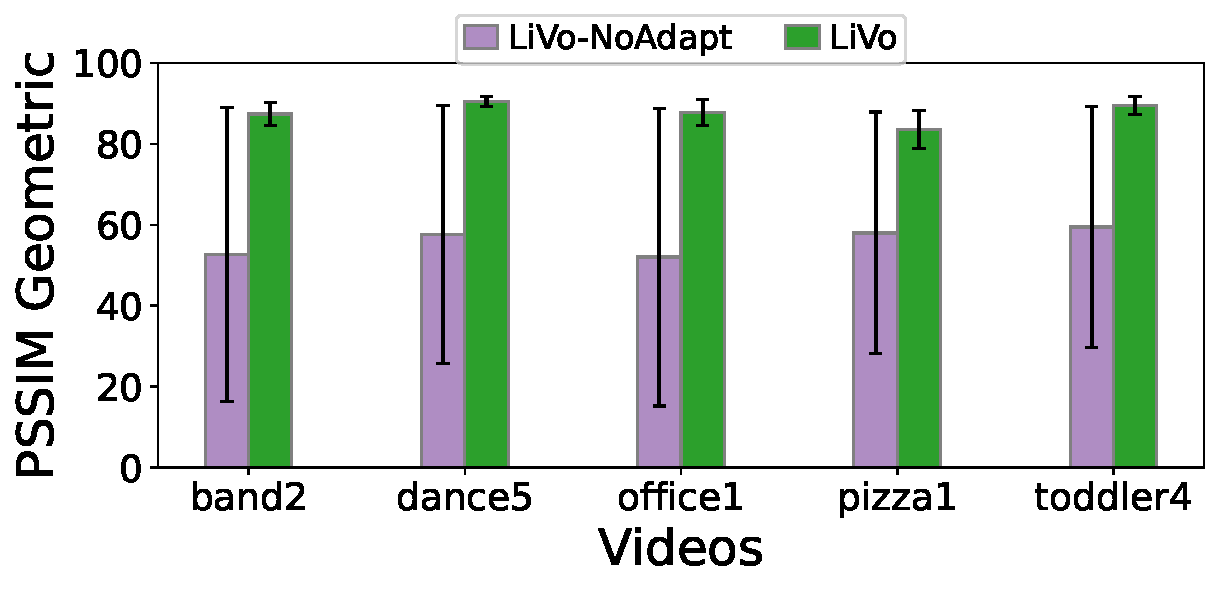
\includegraphics[width=\columnwidth]{figures/pssim_geo_starline_livo.pdf}
%          \caption{Geometry}
%          \label{plot:pssim_geo_starline_livo}
%      \end{subfigure}
%      \hfill
%      \begin{subfigure}[b]{0.49\columnwidth}
%          \centering
%          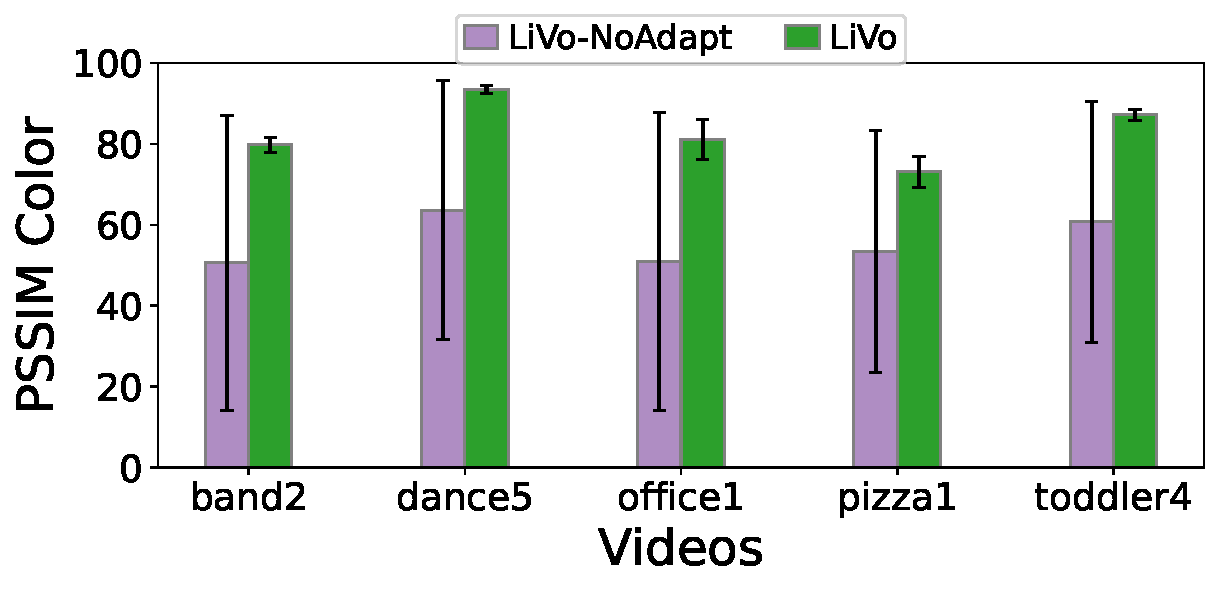
\includegraphics[width=\columnwidth]{figures/pssim_color_starline_livo.pdf}
%          \caption{Color}
%          \label{plot:pssim_color_starline_livo}
%      \end{subfigure}
%     \caption{PSSIM metric for Starline (no adaptation) vs \sysname}
%     \label{plot:pssim_starline_livo}
% \end{figure}
%
\begin{figure}[t]
  \begin{minipage}[t]{0.49\columnwidth}
    \centering
     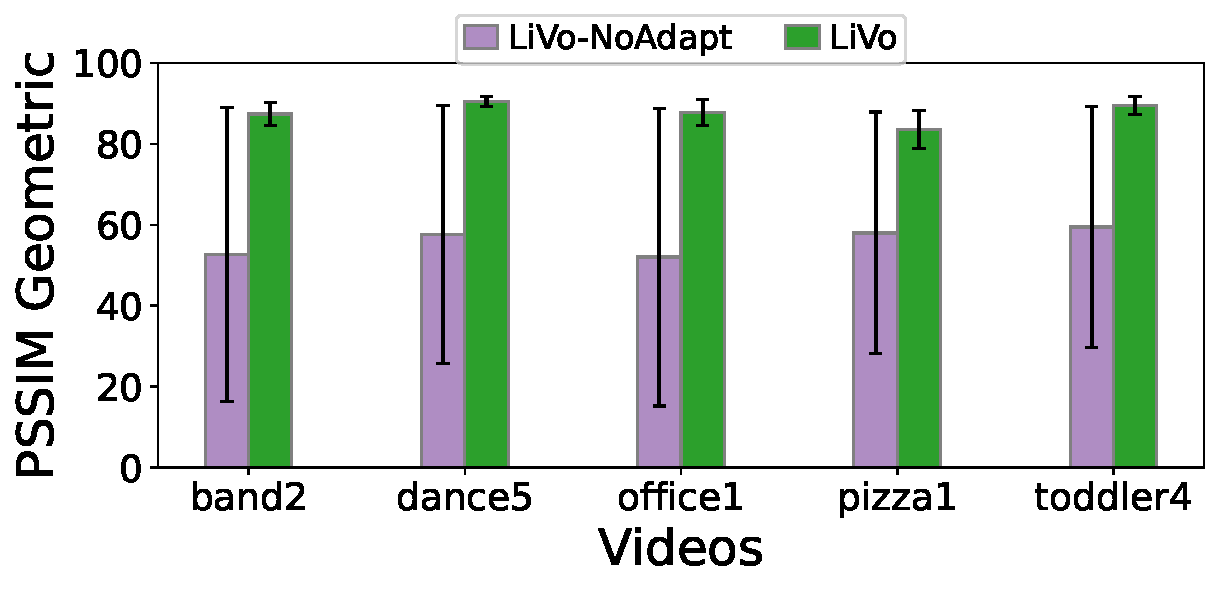
\includegraphics[width=\columnwidth]{figures/pssim_geo_starline_livo.pdf}
    \caption{PSSIM Geometric, \sysname-NoAdapt vs \sysname.}
    \label{plot:pssim_geo_starline_livo}
  \end{minipage}
  \begin{minipage}[t]{0.49\columnwidth}
    \centering
     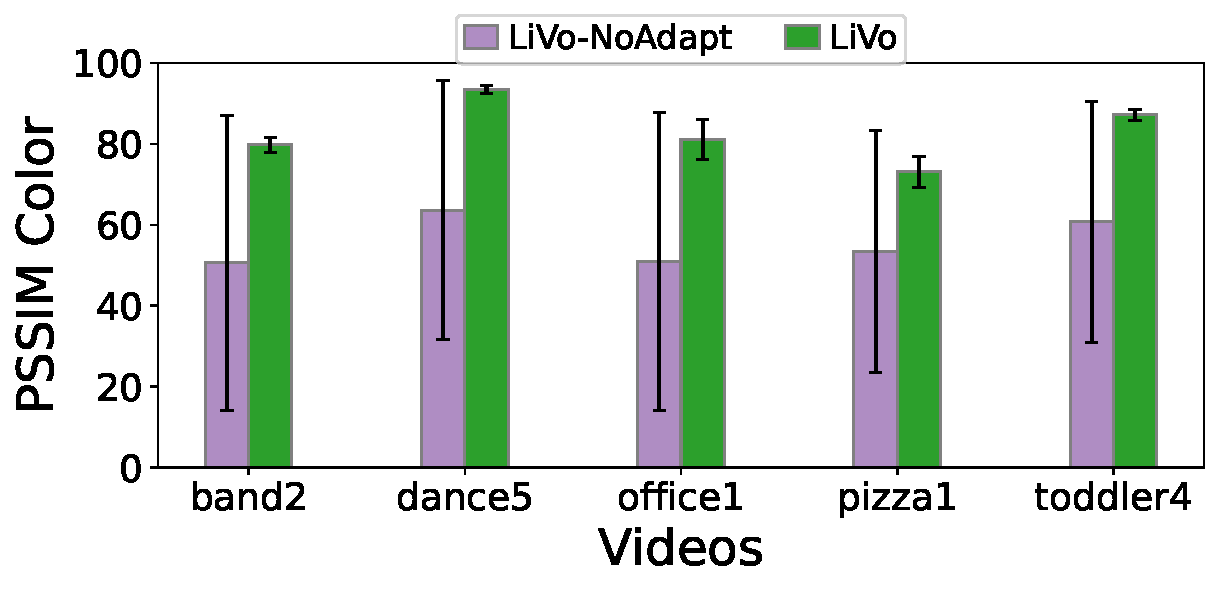
\includegraphics[width=\columnwidth]{figures/pssim_color_starline_livo.pdf}
    \caption{PSSIM Color, \sysname-NoAdapt vs \sysname.}
    \label{plot:pssim_color_starline_livo}
  \end{minipage}
\end{figure}
%
What if LiVo did not use bandwidth-adaptation and view culling at all, but instead used fixed quality parameters?
%
We set fixed color QP (quantization parameter) to 22 and depth QP to 14; Starline~\cite{starline} uses these values.
%
\cref{plot:pssim_geo_starline_livo} and \cref{plot:pssim_color_starline_livo} show that this LiVo-NoAdapt has significant quality drop of $30-41\%$ for geometry and $27-37\%$ for color, with PSSIM going below 60.

\parab{Frustum Prediction.}
%
\begin{table}[t]
\centering
\footnotesize
    \scalebox{0.8}
    {
	\begin{tabular}{|l|l|l|l|}
		\hline
		\textbf{Method} & \textbf{\begin{tabular}[c]{@{}l@{}}\# Hidden \\ Units\end{tabular}} & \textbf{\begin{tabular}[c]{@{}l@{}}Position \\ (m)\end{tabular}} & \textbf{\begin{tabular}[c]{@{}l@{}}Rotation \\ (degree)\end{tabular}} \\ \hline
		\multirow{3}{*}{\begin{tabular}[c]{@{}l@{}}MLP\\ Trained on \\ 1 user trace\end{tabular}} & 3 & 1.01 & 135.86 \\ \cline{2-4} 
		& 32 & 0.59 & 80.46 \\ \cline{2-4} 
		& 64 & 0.24 & 58.24 \\ \hline
		\multirow{3}{*}{\begin{tabular}[c]{@{}l@{}}MLP\\ Trained on\\ 2 user trace\end{tabular}} & 3 & 0.40 & 33.34 \\ \cline{2-4} 
		& 32 & 0.09 & 3.69 \\ \cline{2-4} 
		& 64 & 0.07 & 2.17 \\ \hline
		Kalman Filter & - & 0.04 & 7.19 \\ \hline
	\end{tabular}
    }
	\caption{Comparing prediction errors in Kalman Filter-based to learning-based prediction methods.} % For band2 video
	\label{tab:frustum_kf_learning}
\end{table}
%
To estimate quality impairment as a result of our predictive culling, we compare it against LiVo with perfect culling (using predictions obtained from the user trace).
%
The average quality difference in PSSIM geometry and color is $1\%$ across all 5 videos when run on \textit{trace-1}.

Prior work has trained frustum predictors from user traces~\cite{vues,vivo} for on-demand volumetric videos.
%
This doesn't quite apply to conferencing, since user interactions depend on content, which can be different for different content.
%
That said, we evaluate (\cref{tab:frustum_kf_learning}) whether an MPL with 3 hidden layers used in ViVo~\cite{vivo} could learn from a small number of our traces.
%
We find that it may be possible to match LiVo's predictor only with a large number of hidden layers (64); with the three that ViVo uses, prediction errors are unacceptably high.


% \begin{figure}[t]
%      \centering
%      \begin{subfigure}[b]{0.9\columnwidth}
%          \centering
%     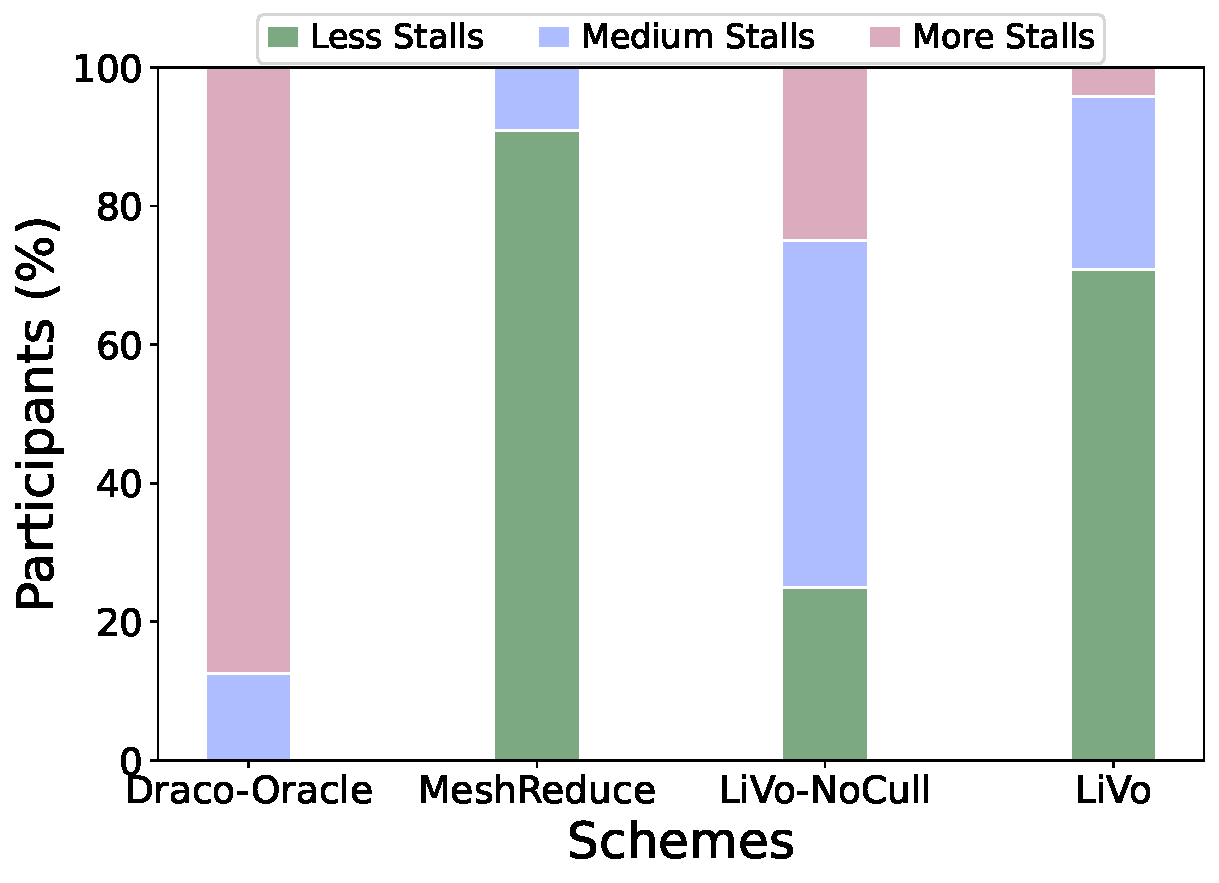
\includegraphics[width=\columnwidth]{figures/user_study_stall_distribution.pdf}
%     \caption{Feedback on stalls}
%     \label{plot:user_study_stalls}
%      \end{subfigure}
%      \hfill
%      \begin{subfigure}[b]{0.9\columnwidth}
%          \centering
%          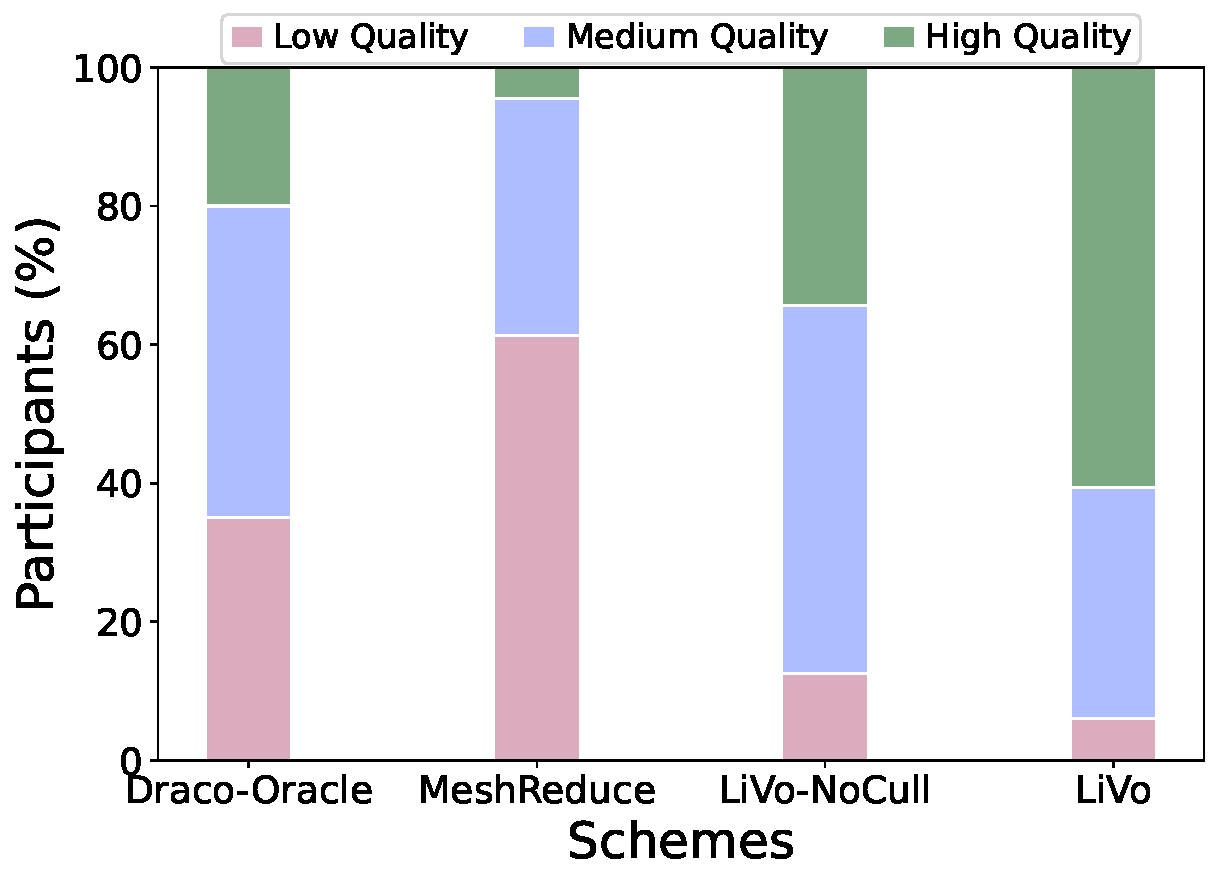
\includegraphics[width=\columnwidth]{figures/user_study_quality_distribution.pdf}
%     \caption{Feedback on quality.}
%     \label{plot:user_study_quality}
%      \end{subfigure}
%      \hfill
%      \begin{subfigure}[b]{0.9\columnwidth}
%          \centering
%          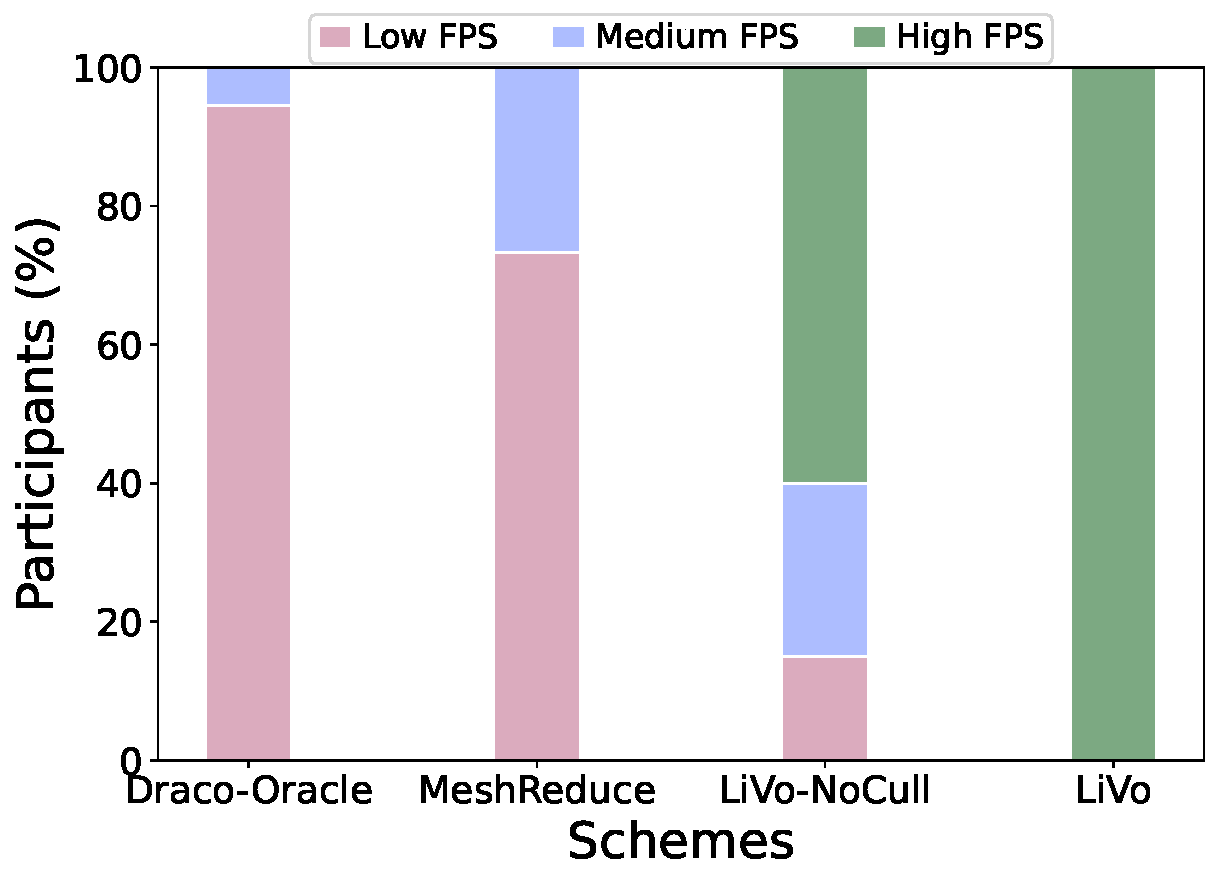
\includegraphics[width=\columnwidth]{figures/user_study_fps_distribution.pdf}
%     \caption{Feedback on fps.}
%     \label{plot:user_study_fps}
%      \end{subfigure}
%         \caption{Summary of user feedback.}
%         \label{plot:user_study_summary}
% \end{figure}

\subsection{Depth vs Color Distortion}
\cref{plot:bitrate-distortion} studies variability in PSSIM quality metric in depth (sim. color) when we fix color (sim. depth) bitrate and vary depth bitrate. \cref{plot:depth-distortion} shows how PSSIM Geometry metric varies when we increase depth bitrate (normalized as depth bitrate per point); similarly report PSSIM color in \cref{plot:color-distortion}. We observe that depth varies a lot with increase in bitrate before it flattens, while variation in color quality is minimal. Also, the bitrate that needs be allocated for depth is almost $7\times$ higher before it saturates (around vertical dotted line). This confirms that depth is much more sensitive to color and needs careful bitrate allocation.
%
\begin{figure}[t]
    \centering
    \begin{subfigure}[b]{0.49\columnwidth}
         \centering
         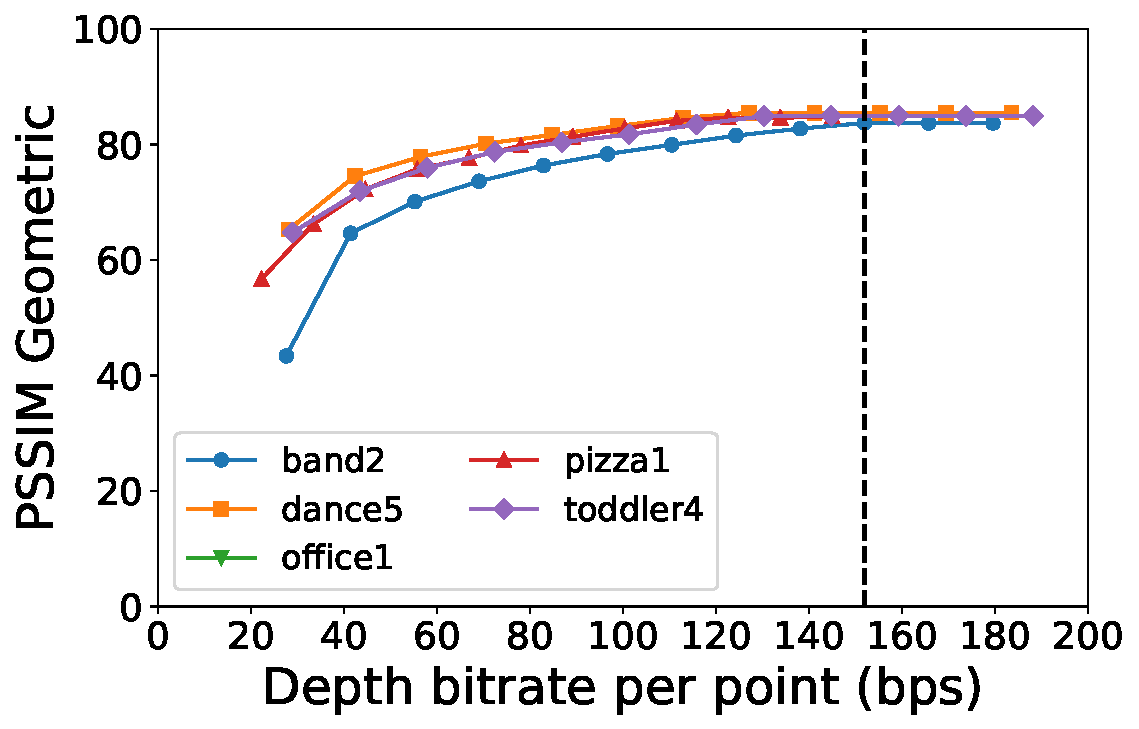
\includegraphics[width=\columnwidth]{figures/pssim_geometric_depth_per_point.pdf}
        \caption{Depth distortion vs depth bitrate.}
        \label{plot:depth-distortion}
    \end{subfigure}
    \hfill
    \begin{subfigure}[b]{0.49\columnwidth}
         \centering
         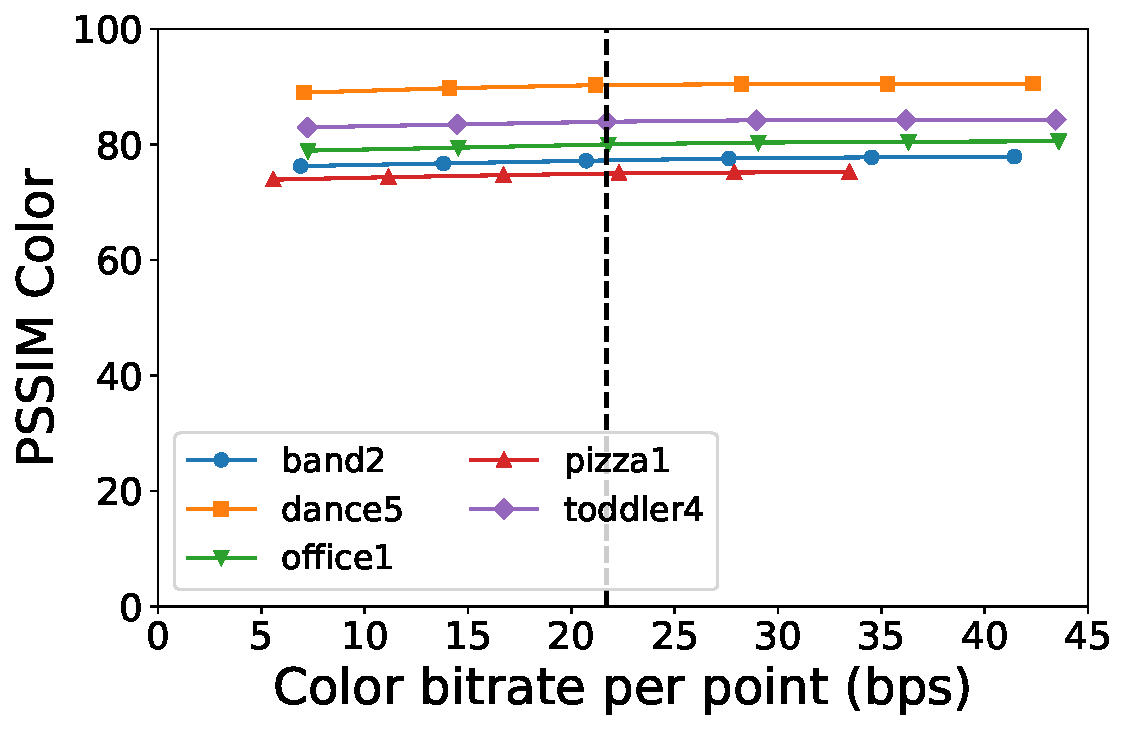
\includegraphics[width=\columnwidth]{figures/pssim_color_color_per_point.pdf}
        \caption{Color distortion vs color bitrate.}
        \label{plot:color-distortion}
    \end{subfigure}
    \caption{PSSIM distortion across videos when bitrate is varied}
    \label{plot:bitrate-distortion}
\end{figure}

\subsection{Variability in Bandwidth Traces}
\label{ss:trace_variability}

We show the variability in the 2 traces we pick - \textit{trace-1} and \textit{trace-2} in \cref{plot:mahimahi_traces}.
\begin{figure}[ht!]
  \centering 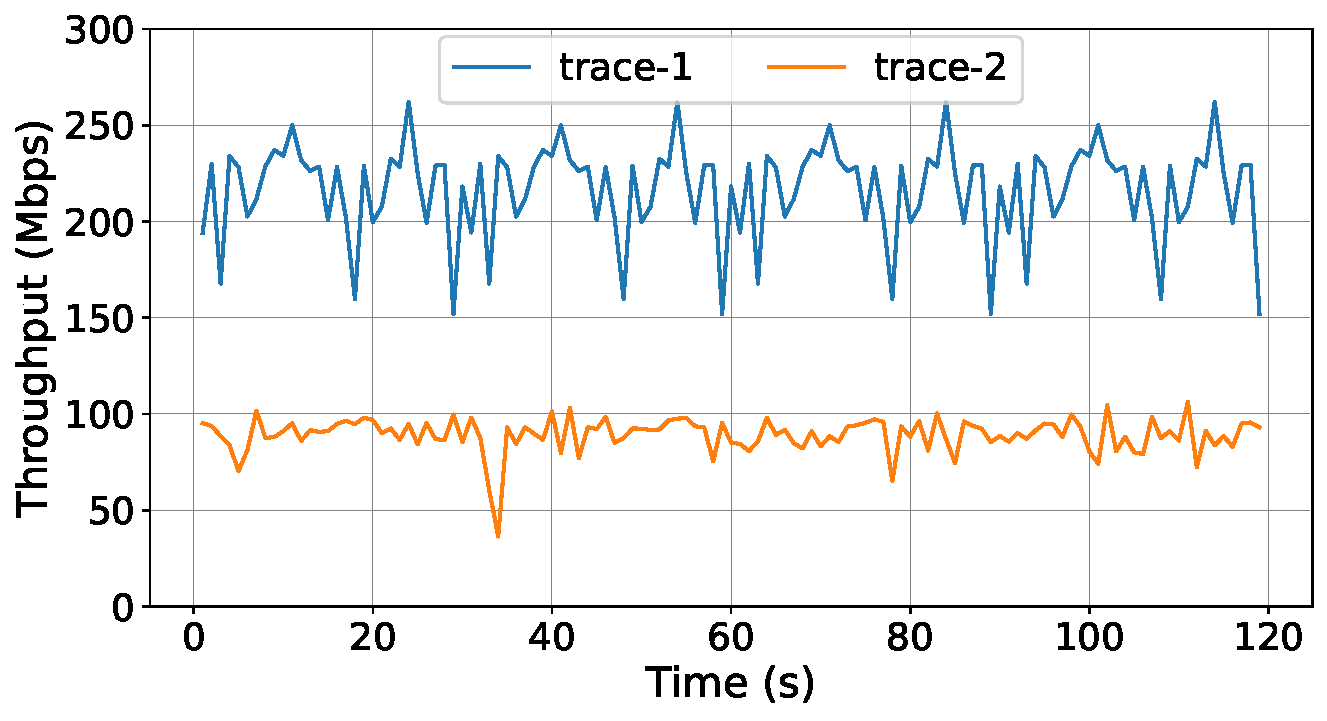
\includegraphics[width=\columnwidth]{figures/throughput_wifi25_tracep1.pdf}
  \caption{Variability in the 2 network traces we consider.}
  \label{plot:mahimahi_traces}
\end{figure}

%
%
% \begin{figure*}[h!]
%   \begin{minipage}[t]{0.33\textwidth}
%     \centering
%     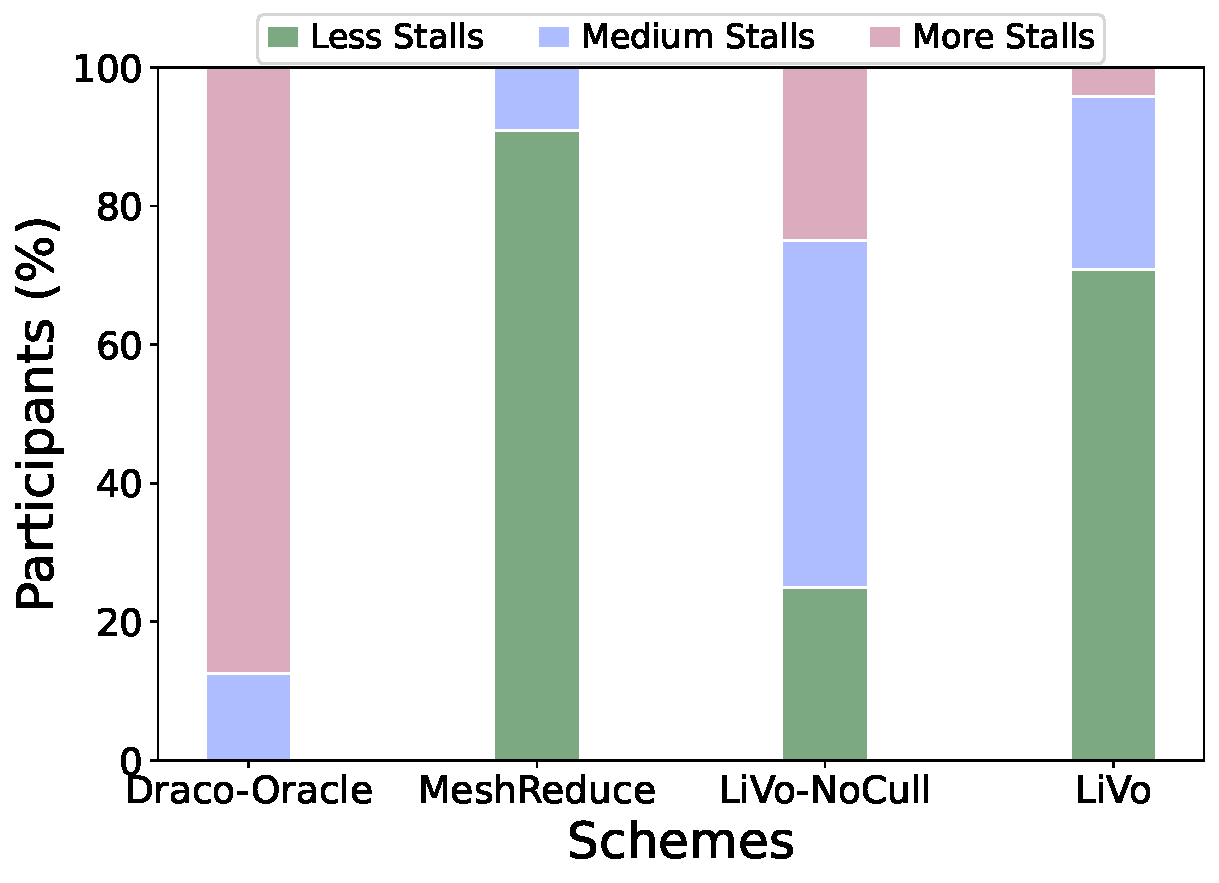
\includegraphics[width=\columnwidth]{figures/user_study_stall_distribution.pdf}
%     \caption{Feedback on stalls}
%     \label{plot:user_study_stalls}
%   \end{minipage}
%   \begin{minipage}[t]{0.33\textwidth}
%     \centering
%     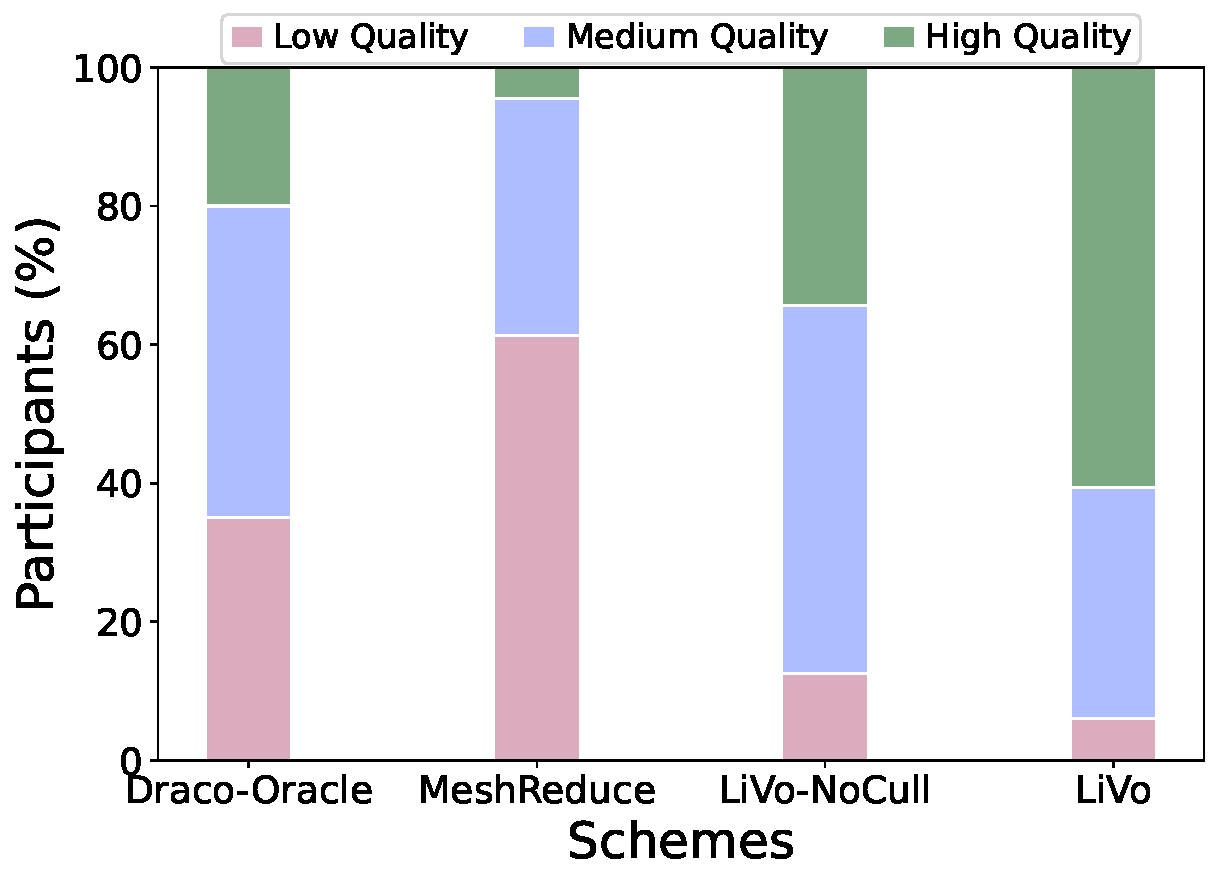
\includegraphics[width=\columnwidth]{figures/user_study_quality_distribution.pdf}
%     \caption{Feedback on quality.}
%     \label{plot:user_study_quality}
%   \end{minipage}
%   \begin{minipage}[t]{0.33\textwidth}
%     \centering 
%     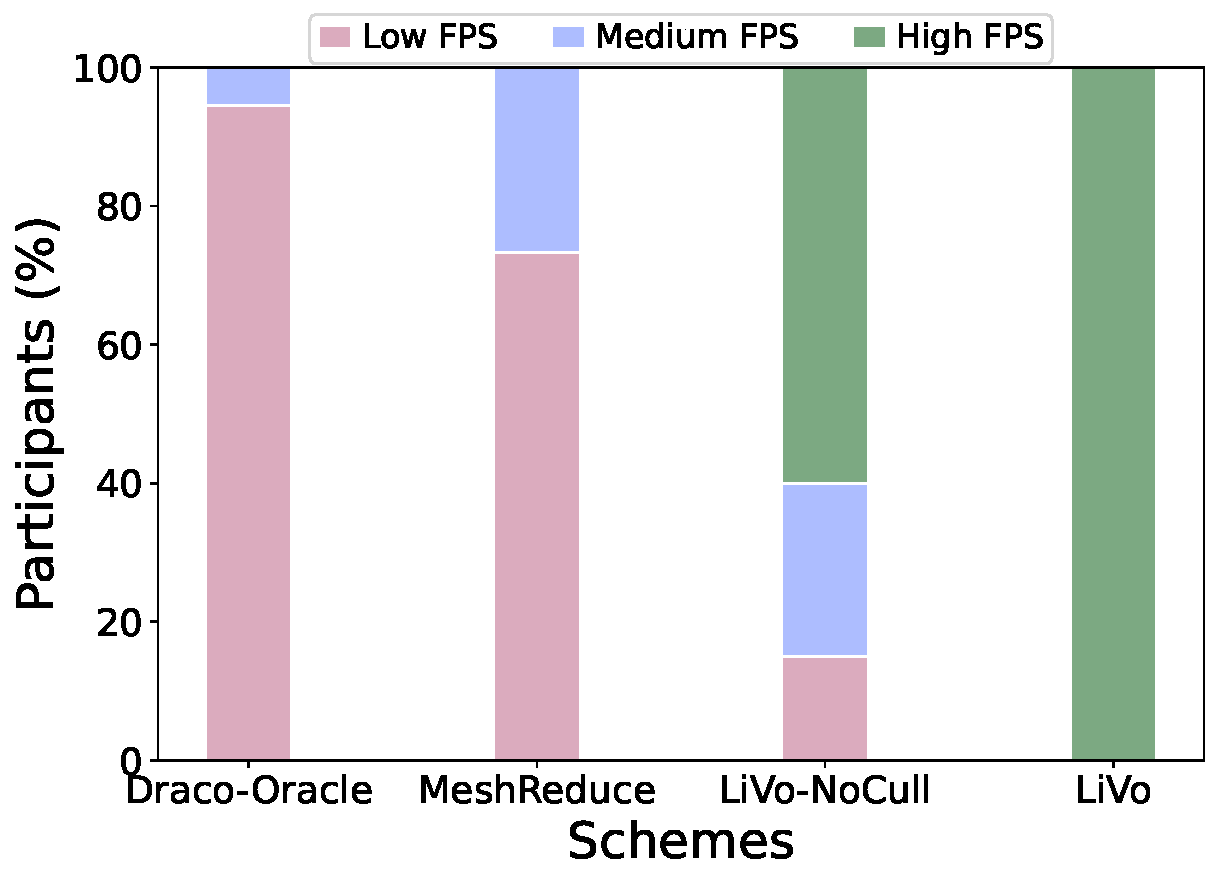
\includegraphics[width=\columnwidth]{figures/user_study_fps_distribution.pdf}
%     \caption{Feedback on FPS.}
%     \label{plot:user_study_fps}
%   \end{minipage}
% \end{figure*}
%
%
